\documentclass[border=10pt,tikz]{standalone}
\usepackage{tikz}
\usetikzlibrary{positioning,arrows.meta}
\begin{document}
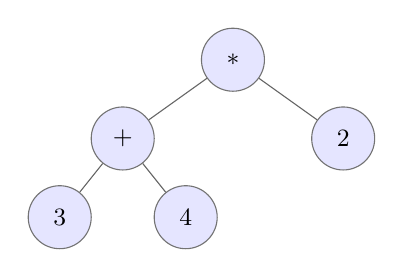
\begin{tikzpicture}[
  font=\sffamily\small,
  every node/.style={circle, draw=black!55, line width=0.4pt, minimum size=8mm, fill=blue!10, inner sep=0pt},
  edge/.style={draw=black!60, line width=0.4pt}
]
\node (root) at (0, 2)    {$*$};
\node (plus) at (-1.4, 1) {$+$};
\node (two)  at (1.4, 1)  {$2$};
\node (three) at (-2.2, 0){$3$};
\node (four)  at (-0.6, 0){$4$};

\draw[edge] (root) -- (plus);
\draw[edge] (root) -- (two);
\draw[edge] (plus) -- (three);
\draw[edge] (plus) -- (four);
\end{tikzpicture}
\end{document}
